\documentclass[a4paper, 11pt]{article}
\usepackage{graphicx,wrapfig,subfigure,amsmath,amssymb,epsfig,bm}
\usepackage{listings,textcomp,color,geometry}
\geometry{hmargin=2cm, vmargin=2cm}
\usepackage[dvipsnames]{xcolor}
\usepackage{amsmath}
\usepackage{tikz}


\def\Box{\mathord{\dalemb{7.9}{8}\hbox{\hskip1pt}}}
\def\dalemb#1#2{{\vbox{\hrule height.#2pt
        \hbox{\vrule width.#2pt height#1pt \kern#1pt \vrule width.#2pt}
        \hrule height.#2pt}}}

\def\eop{\mathcal{E}}
\def\bop{\mathcal{B}}
\def\ba{\begin{eqnarray}}
\def\ea{\end{eqnarray}}
\def\be{\begin{equation}}
\def\ee{\end{equation}}
\def\tr{{\rm tr}}
\def\Var{{\rm Var}}
\def\gtorder{\mathrel{\raise.3ex\hbox{$>$}\mkern-14mu
             \lower0.6ex\hbox{$\sim$}}}
\def\ltorder{\mathrel{\raise.3ex\hbox{$<$}\mkern-14mu
             \lower0.6ex\hbox{$\sim$}}}

\def\bb{{\mathfrak b}}
\newcommand{\ellb }{\boldsymbol{\ell }}

\definecolor{denim}{rgb}{0.08, 0.38, 0.74}
\definecolor{ao}{rgb}{0.0, 0.5, 0.0}

% Personal colors defined here
\newcommand{\red}[1]{{\color{red}#1}}
\newcommand{\green}[1]{{\color{ForestGreen}#1}}
\newcommand{\cyan}[1]{{\color{Orange}#1}}
\newcommand{\blue}[1]{{\color{denim}#1}}
\newcommand{\assume}[1]{{\bf#1}}

\begin{document}

\begin{figure}
  \centering
  \includegraphics[width=1\columnwidth]{lensing.png}
  \caption{Path of a light ray from the last scattering surface to us.  (left) assuming no lensing, (right) the light ray is lensed by a mass in the lens plane.}
  \label{fig:scanningstrat}
\end{figure}



\section{The comoving distance }

The homogeneous FLRW universe is described by the following metric
\ba
ds^{2} = -c^{2}dt^{2} + a^{2}\delta_{ij}dx^{i}dx^{j}
\ea
The metric describes an expanding Universe with scale factor $a$, $a$ serves to stretch the fixed grid defined by the coordinate $x^{i}$, we say that the coordinate $x^{i}$ are comoving, they are not affected by the Universe dynamics. 
Let's consider the path of a radial light ray, we use $\chi$ here as a radial comoving coordinate
\ba
ds^{2} = -c^{2}dt^{2} + a^{2}d\chi^{2} = 0 
\ea

If an object that emit light at $t_{e}$ and with receive it at $t_{0}$, and if we assume that we are at the center of the coordinate system, the object is at comoving coordinate
\ba
\chi = \int_{t_{e}}^{t_{0}} \frac{c dt}{a(t)}
\ea
note that a(t) is an increasing function of time, and $t_{0} > t$ so $\chi$ here is positive.

The comoving distance can be expressed in term of scale factor 
\ba
\chi = \int_{t_{e}}^{t_{0}} \frac{c dt}{a} =  \int_{a_{e}}^{1} \frac{c da}{a} \frac{dt}{da} = \int_{a_{e}}^{1}  \frac{c da}{ H(a) a^{2}} 
\ea
using $H = \frac{da/dt}{a}$, and $a(t_{0}) = 1$ or as a function of redshift using $a = \frac{1}{1+z}$
\ba
\frac{da}{dz} = - \left(\frac{1}{1+z}\right)^{2}= -a^{2}
\ea

\ba
\chi  = \int_{a_{e}}^{1}  \frac{c da}{ H(a) a^{2}} = \int^{z_{e}}_{0}  \frac{c dz}{ H(z)}
\ea



\section{The lensing potential}

The true position of the source is at location 
\ba
\bm{x}_{\rm true}  =\chi_{\rm LSS} \begin{pmatrix} 
{\theta}^{1}_{S} \cr
{\theta}^{2}_{S} \cr
 1
 \end{pmatrix} 
\ea
Where $\theta^{1}_{S}, \theta^{2}_{S}$ are small quantities in our reference frame, its apparent location is $\bm{x}_{\rm obs} = \chi_{\rm LSS}  \begin{pmatrix} 
{\theta}^{1} \cr
{\theta}^{2} \cr
 1
 \end{pmatrix} $
 , we need to relate ${\theta}^{i}_{S}$  to ${\theta}^{i}$. 
We will work in the perturbed FLRW metric in Newtonian gauge
\ba
ds^{2} = -(1 + 2\psi(\bm{x},t))dt^{2} + a^{2}(t)\delta_{ij}[1+2\phi(\bm{x},t)]dx^{i}dx^{j}
\ea


which has the following non zero Christoffel symbol
\ba
\Gamma^{0}_{00} &=& \dot{\psi} \\
\Gamma^{i}_{j0}  &=& \delta^{i}_{j} (H +\dot{\phi}) \\
\Gamma^{i}_{00}  &=& \partial^{i} \psi \\
\Gamma^{i}_{jk} &=&   (\delta^{i}_{j} \partial_{k} - \delta^{i}_{k} \partial_{j}  - \delta^{im}\delta_{jk} \partial_{m} ) \phi
\ea
we will study the path of photon, we have the following condition for their four-momentum $P^{\mu} = \frac{dx^{\mu}}{d\lambda}$: $P^{\mu}P_{\mu} = 0$, defining $p = g_{ij}P^{i}P^{j}$
\ba
 &&-(1 + 2\psi(\bm{x},t))(P^{0})^{2} + p^{2} = 0 \\
 &&\frac{dt}{d\lambda}  = P^{0} \approx p(1-\psi) \\
\ea

The geodesic equation is 
\ba
\frac{d^{2} x^{\rho}}{d\lambda^{2}} &=& -\Gamma^{\rho}_{\mu, \nu} \frac{dx^{\mu}}{d\lambda} \frac{dx^{\nu}}{d\lambda} 
\ea
with 1 and 2 components
\ba
\frac{d^{2}(\chi \theta^{i}) }{d\lambda^{2}} &=& -\Gamma^{i}_{\mu, \nu} \frac{dx^{\mu}}{d\lambda} \frac{dx^{\nu}}{d\lambda} 
\ea
let's first expand the left hand side, 
\ba
\frac{d^{2}(\chi \theta^{i}) }{d\lambda^{2}} &=& \frac{d}{d\lambda} \left(\frac{d(\chi \theta^{i}) }{d\lambda}\right) \\
&=& \frac{d}{d\lambda} \left(\frac{d(\chi \theta^{i}) }{d\chi}\frac{d\chi}{dt} \frac{dt}{d\lambda} \right)  \\
&= & \frac{d\chi}{dt} \frac{dt}{d\lambda} \frac{d}{d\chi} \left(\frac{d(\chi \theta^{i}) }{d\chi}\frac{d\chi}{dt} \frac{dt}{d\lambda} \right)
\ea
Now let's expand the right hand side
\ba
 -\Gamma^{i}_{\mu, \nu} \frac{dx^{\mu}}{d\lambda} \frac{dx^{\nu}}{d\lambda} = -\Gamma^{i}_{\mu, \nu} \frac{dx^{\mu}}{d\chi} \frac{dx^{\nu}}{d\chi}  \left(\frac{d\chi}{dt}\right)^{2} \left(\frac{dt}{d\lambda} \right)^{2}
\ea
putting this together we have
\ba
\frac{d}{d\chi} \left(\frac{d(\chi \theta^{i}) }{d\chi}\frac{d\chi}{dt} \frac{dt}{d\lambda} \right) &=& -\Gamma^{i}_{\mu, \nu} \frac{dx^{\mu}}{d\chi} \frac{dx^{\nu}}{d\chi}  \frac{d\chi}{dt} \frac{dt}{d\lambda} \\
\frac{d}{d\chi} \left(\frac{d(\chi \theta^{i}) }{d\chi}\frac{d\chi}{dt} \frac{dt}{d\lambda} \right) &=& - \left[\Gamma^{i}_{0,0} \left(\frac{dx^{0}}{d\chi}\right)^{2} + 2 \Gamma^{i}_{0,j} \frac{dx^{0}}{d\chi}\frac{dx^{j}}{d\chi}  + \Gamma^{i}_{j,k}\frac{dx^{j}}{d\chi} \frac{dx^{k}}{d\chi}   \right]  \frac{d\chi}{dt} \frac{dt}{d\lambda} 
\ea

at zero order, we have $ d\chi = -d\eta = - \frac{dt}{a}$ and $\frac{dt}{d\lambda} = p$, we will also use that $\frac{d(\chi \theta^{i}) }{d\chi}$ is a small quantity, 
\ba
\frac{d(\chi \theta^{i}) }{d\chi} = \theta^{i} + \chi \frac{d \theta^{i} }{d\chi}
\ea
$\theta^{i}$ is small and $\frac{d \theta^{i} }{d\chi}$ is of order of the gravitational potential perturbation (since it's zero with no grav lensing effect).

\ba
\frac{d}{d\chi} \left( -\frac{p}{a}\frac{d(\chi \theta^{i}) }{d\chi} \right) &=& \frac{p}{a} \left[ a^{2}  \partial^{i} \psi - 2 a H \frac{d(\chi \theta^{i}) }{d\chi}  + \Gamma^{i}_{j,k}\frac{dx^{j}}{d\chi} \frac{dx^{k}}{d\chi}   \right] 
\ea
\ba
\Gamma^{i}_{j,k}\frac{dx^{j}}{d\chi} \frac{dx^{k}}{d\chi} = \Gamma^{i}_{3,3} =  -\delta^{im}\partial_{m} \phi
\ea
because the $\frac{dx^{i}}{d\chi}$ for $i \in (1,2)$ is first order in perturbation while $\frac{dx^{3}}{d\chi} = 1$
\ba
\frac{d}{d\chi} \left( -\frac{p}{a}\frac{d(\chi \theta^{i}) }{d\chi} \right) &=& \frac{p}{a} \left[ a^{2}  \partial^{i} \psi - 2 a H \frac{d(\chi \theta^{i}) }{d\chi}   -\delta^{im}\partial_{m} \phi  \right] 
\ea


We know that at 0th order, $p = \frac{C}{a}$ with C = cst
\ba
\frac{d}{d\chi} \left( \frac{1}{a^{2}}\frac{d(\chi \theta^{i}) }{d\chi} \right) &=& -\frac{1}{a^{2}} \left[ a^{2}  \partial^{i} \psi - 2 a H \frac{d(\chi \theta^{i}) }{d\chi}   -\delta^{im}\partial_{m} \phi  \right]  \nonumber \\
\frac{d}{d\chi} \left( \frac{1}{a^{2}}\frac{d(\chi \theta^{i}) }{d\chi} \right) &=& -\left[  \partial^{i} \psi - \frac{2}{a}  H \frac{d(\chi \theta^{i}) }{d\chi}   -\partial^{i} \phi  \right] \nonumber \\
\frac{d}{d\chi} \left( \frac{1}{a^{2}}\frac{d(\chi \theta^{i}) }{d\chi} \right) &=& -\left[  \partial^{i} (\psi -\phi) - \frac{2}{a}  H \frac{d(\chi \theta^{i}) }{d\chi}     \right] 
\ea
Where I use the homogenous FLRW metric to raise the index in the third term of the right hand side.
We can expand the left hand side
\ba
\frac{d}{d\chi} \left( \frac{1}{a^{2}}\frac{d(\chi \theta^{i}) }{d\chi} \right)  &=& \frac{1}{a^{2}} \frac{d^{2}(\chi \theta^{i}) }{d\chi^{2}} +\frac{d a^{-2}}{d\chi}  \frac{d(\chi \theta^{i}) }{d\chi} \nonumber \\
\frac{d}{d\chi} \left( \frac{1}{a^{2}}\frac{d(\chi \theta^{i}) }{d\chi} \right)  &=& \frac{1}{a^{2}} \frac{d^{2}(\chi \theta^{i}) }{d\chi^{2}}  - \frac{2}{a^{3}}  \frac{d a}{dt}\frac{dt}{d\chi}  \frac{d(\chi \theta^{i}) }{d\chi} \nonumber \\
\frac{d}{d\chi} \left( \frac{1}{a^{2}}\frac{d(\chi \theta^{i}) }{d\chi} \right)  &=& \frac{1}{a^{2}} \frac{d^{2}(\chi \theta^{i}) }{d\chi^{2}}  +\frac{2 H}{a}    \frac{d(\chi \theta^{i}) }{d\chi} 
\ea
Finally
\ba
 \frac{d^{2}(\chi \theta^{i}) }{d\chi^{2}}   &=&  -a^{2} \left[  \partial^{i} (\psi -\phi)  \right] \\
 &=& - \delta^{ij} \partial_{j} (\psi -\phi)
\ea
We can integrate this equation with respect to $\chi$
\ba
 \frac{d(\chi \theta^{i}) }{d\chi} &=&  - \delta^{ij} \int^{\chi}_{0} \partial_{j} [\psi(\bm{x}(\bm{\theta}, \chi_{1}), \eta_{0}-\chi_{1}) -\phi(\bm{x}(\bm{\theta}, \chi_{1}), \eta_{0}-\chi_{1})]  d\chi_{1} + C^{i}_{1} \\
\ea

\begin{figure}
    \begin{minipage}{0.5\textwidth}
        \centering
        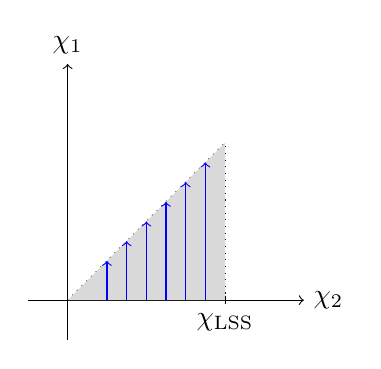
\begin{tikzpicture}[scale=0.5]
            % Draw axes
            \draw[->] (-1,0) -- (6,0) node[right] {$\chi_2$};
            \draw[->] (0,-1) -- (0,6) node[above] {$\chi_1$};
            
             \draw[dotted] (0,0) -- (4,4) node[right]{};
             \draw[dotted] (4,0) -- (4,4) node[right]{};
    
    	      \fill[gray!30] (0,0) -- (4,0) -- (4,4) -- cycle;
	      
              \draw[blue, ->] (1,0) -- (1,1) node[right]{};
              \draw[blue, ->] (1.5,0) -- (1.5,1.5) node[right]{};
	     \draw[blue, ->] (2,0) -- (2,2) node[right]{};
	      \draw[blue, ->] (2.5,0) -- (2.5,2.5) node[right]{};
	      \draw[blue, ->] (3,0) -- (3,3) node[right]{};
	      \draw[blue, ->] (3.5,0) -- (3.5,3.5) node[right]{};

    
            % Draw tick and label for x-coordinate
            \draw (4,0.1) -- (4,-0.1) node[below] {$\chi_{\rm LSS}$};
            
            % Draw frame
        \end{tikzpicture}
        \label{fig:frame_left}
    \end{minipage}%
    \begin{minipage}{0.5\textwidth}
        \centering
        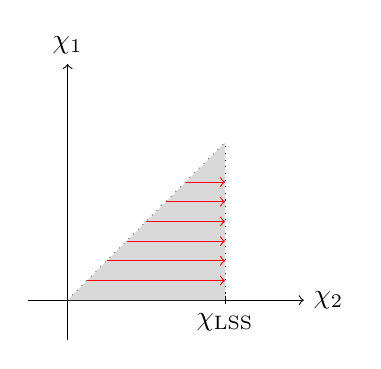
\begin{tikzpicture}[scale=0.5]
            % Draw axes
            \draw[->] (-1,0) -- (6,0) node[right] {$\chi_2$};
            \draw[->] (0,-1) -- (0,6) node[above] {$\chi_1$};
            
             \draw[dotted] (0,0) -- (4,4) node[right]{};
             \draw[dotted] (4,0) -- (4,4) node[right]{};
    
    	      \fill[gray!30] (0,0) -- (4,0) -- (4,4) -- cycle;
	      
	       \draw[red, ->] (0.5,0.5) -- (4,0.5) node[right]{};
              \draw[red, ->] (1,1) -- (4,1) node[right]{};
    	     \draw[red, ->] (1.5,1.5) -- (4,1.5) node[right]{};
              \draw[red, ->] (2,2) -- (4,2) node[right]{};
              \draw[red, ->] (2.5,2.5) -- (4,2.5) node[right]{};
	      \draw[red, ->] (3,3) -- (4,3) node[right]{};

	      
            % Draw tick and label for x-coordinate
            \draw (4,0.1) -- (4,-0.1) node[below] {$\chi_{\rm LSS}$};
            
            % Draw frame
        \end{tikzpicture}
        \label{fig:frame_right}
    \end{minipage}
    \caption{Two different way of doing the integration of $f(\chi_{1}, \chi_{2})$ over the triangle area, the inner integral is shown in lines. On the left $\int^{\chi_{\rm LSS}}_{0} d\chi_{2} \int^{\chi_{2}}_{0} d\chi_{1}f(\chi_{1}, \chi_{2})$, on the right $\int^{\chi_{\rm LSS}}_{0} d\chi_{1} \int^{\chi_{\rm LSS}}_{\chi_{1}} d\chi_{2}f(\chi_{1}, \chi_{2})$ }  
    \label{fig:frame}
\end{figure}

We can then integrate again from 0 to the last scattering surface 
\ba
\chi_{\rm LSS} \theta^{i}(\chi_{\rm LSS}) &=&  - \delta^{ij}  \int^{\chi_{\rm LSS}}_{0} d \chi_{2} \int^{\chi_{2}}_{0} \partial_{j} [\psi(\bm{x}(\bm{\theta}, \chi_{1}), \eta_{0}-\chi_{1}) -\phi(\bm{x}(\bm{\theta}, \chi_{1}), \eta_{0}-\chi_{1})]  d\chi_{1} + C^{i}_{1}\chi_{ \rm LSS} \nonumber
\ea
nothing that $\theta^{i}(\chi_{\rm LSS}) = \theta^{i}_{S}$
\ba
 \theta^{i}_{S} =  - \frac{\delta^{ij}  }{\chi_{\rm LSS} } \int^{\chi_{\rm LSS}}_{0} d \chi_{2} \int^{\chi_{2}}_{0} \partial_{j} [\psi( \bm{x}(\bm{\theta}, \chi_{1}), \eta_{0}-\chi_{1}) -\phi( \bm{x}(\bm{\theta}, \chi_{1}), \eta_{0}-\chi_{1})]  d\chi_{1} + C^{i}_{1}
\ea
in the absence of gravitational potential $ \theta^{i}_{S} =  \theta^{i}$ so $C^{i}_{1} = \theta^{i}$ .
\ba
 \theta^{i}_{S} =  \theta^{i} - \frac{\delta^{ij}  }{\chi_{\rm LSS} } \int^{\chi_{\rm LSS} }_{0} d \chi_{2} \int^{\chi_{2}}_{0} \partial_{j} [\psi( \bm{x}(\bm{\theta}, \chi_{1}), \eta_{0}-\chi_{1}) -\phi( \bm{x}(\bm{\theta}, \chi_{1}), \eta_{0}-\chi_{1})]  d\chi_{1} 
\ea
As shown on Fig \ref{fig:frame}, we can invert the integration order to make the inner integral trivial
\ba
 \theta^{i}_{S}  &=&  \theta^{i} - \frac{\delta^{ij}  }{\chi_{\rm LSS} } \int^{\chi_{\rm LSS}}_{0} d\chi_{1} \int^{\chi_{\rm LSS}}_{\chi_{1}}  \partial_{j} [\psi( \bm{x}(\bm{\theta}, \chi_{1}), \eta_{0}-\chi_{1}) -\phi( \bm{x}(\bm{\theta}, \chi_{1}), \eta_{0}-\chi_{1})]  d\chi_{2} \\
 \theta^{i}_{S} &=&  \theta^{i} - \delta^{ij}  \int^{\chi_{\rm LSS}}_{0} d\chi_{1} \partial_{j} \left[\psi\left(\bm{x}(\bm{\theta}, \chi_{1}), \eta_{0}-\chi_{1} \right) -\phi \left( \bm{x}(\bm{\theta}, \chi_{1}), \eta_{0}-\chi_{1} \right) \right]  \left(1 - \frac{\chi_{1}}{\chi_{\rm LSS} } \right)  
\ea
assuming $ \psi = - \phi$ 
\ba
 \theta^{i}_{S} &=&  \theta^{i} + 2 \delta^{ij}  \int^{\chi_{\rm LSS}}_{0} d\chi_{1} \partial_{j} \phi \left( \bm{x}(\bm{\theta}, \chi_{1}), \eta_{0}-\chi_{1} \right)  \left(1 - \frac{\chi_{1}}{\chi_{\rm LSS} } \right)  
\ea
this is the formula we were looking for.
\ba
 \theta^{i}_{S}  &=&   \theta^{i} + \Delta  \theta^{i} \\
 \Delta  \theta^{i} &=& 2 \delta^{ij}  \int^{\chi_{\rm LSS}}_{0} d\chi_{1} \partial_{j} \phi \left( \bm{x}(\bm{\theta}, \chi_{1}), \eta_{0}-\chi_{1} \right)  \left(1 - \frac{\chi_{1}}{\chi_{\rm LSS} } \right)  
\ea
We use $\frac{\partial}{\partial x^{j}} = \frac{1}{\chi_{1}} \frac{\partial}{\partial \theta^{j}}$
\ba
 \Delta  \theta^{i} &=& 2 \delta^{ij}  \int^{\chi_{\rm LSS}}_{0} \frac{d\chi_{1}}{\chi_{1}} \frac{\partial \phi}{\partial \theta^{j}}  \left( \bm{x}(\bm{\theta}, \chi_{1}), \eta_{0}-\chi_{1} \right)  \left(1 - \frac{\chi_{1}}{\chi_{\rm LSS} } \right)   \\
  &=& \delta^{ij} \frac{\partial }{\partial \theta^{j}} \phi^{L}(\bm{\theta}) \\
  \phi^{L}(\bm{\theta}) &=&  2 \int^{\chi_{\rm LSS}}_{0} \frac{d\chi_{1}}{\chi_{1}}  \phi \left( \bm{x}(\bm{\theta}, \chi_{1}), \eta_{0}-\chi_{1} \right)  \left(1 - \frac{\chi_{1}}{\chi_{\rm LSS} } \right)
\ea

\section{The lensing power spectrum}

Let's rewrite: $ \phi \left( \bm{x}(\bm{\theta}, \chi_{1}), \eta_{0}-\chi_{1} \right)  = \phi \left( \chi_{1} \bm{\hat{n}}, \eta(\chi_{1}) \right)   $  with $\eta(\chi_{1}) = \eta_{0}- \chi_{1}$ and $\bm{\hat{n}}$ the line of sight. 
In order to get to the lensing power spectrum we will first Fourier transform the gravitational potential term
\ba
\phi \left( \chi_{1} \bm{\hat{n}}, \eta(\chi_{1}) \right)    = \int \frac{d^{3}k}{(2\pi)^{3}} e^{i \bm{k} \bm{\hat{n}} \chi_{1}} \phi \left( \bm{k}, \eta(\chi_{1}) \right) 
 \ea
the lensing potential become
\ba
  \phi^{L}(\bm{\hat{n}}) &=&  2 \int^{\chi_{\rm LSS}}_{0} \frac{d\chi_{1}}{\chi_{1}}  \left(1 - \frac{\chi_{1}}{\chi_{\rm LSS} } \right)  \int \frac{d^{3}k}{(2\pi)^{3}} e^{i \bm{k} \bm{\hat{n}} \chi_{1}} \phi \left( \bm{k}, \eta(\chi_{1}) \right)
\ea
More torture, let's expand the Fourier coefficient in spherical harmonics 
\ba
e^{i \bm{k} \bm{\hat{n} } \chi_{1}}  = 4\pi \sum^{\infty}_{\ell=0} i^{\ell} j_{\ell}(k  \chi_{1}) \sum^{\ell}_{m = -\ell} Y^{*}_{\ell m}(\hat{\bm{k}})Y_{\ell m}(\hat{\bm{n}})
\ea
so that
\ba
  \phi^{L}(\bm{\hat{n}}) &=&  \sum_{\ell, m} 8\pi  i^{\ell} Y_{\ell m}(\hat{n}) \int \frac{d^{3}k}{(2\pi)^{3}}  Y^{*}_{\ell m}(\hat{\bm{k}})  \int^{\chi_{\rm LSS}}_{0} \frac{d\chi_{1}}{\chi_{1}}  \left(1 - \frac{\chi_{1}}{\chi_{\rm LSS} } \right)   j_{\ell}(k  \chi_{1}) \phi \left( \bm{k}, \eta(\chi_{1}) \right) \\
  &=&  \sum_{\ell, m}    \phi^{L}_{\ell m} Y_{\ell m}(\hat{n})
\ea
with 
\ba
 \phi^{L}_{\ell m} =    8\pi  i^{\ell}  \int \frac{d^{3}k}{(2\pi)^{3}}  Y^{*}_{\ell m}(\hat{\bm{k}})  \int^{\chi_{\rm LSS}}_{0} \frac{d\chi_{1}}{\chi_{1}}  \left(1 - \frac{\chi_{1}}{\chi_{\rm LSS} } \right)   j_{\ell}(k  \chi_{1}) \phi \left( \bm{k}, \eta(\chi_{1}) \right)
\ea
the lensing power spectrum is given by
\ba
\langle \phi^{L}_{\ell m} \phi^{L*}_{\ell m} \rangle =    (8\pi)^{2}   \int \frac{d^{3}k}{(2\pi)^{3}}  Y^{*}_{\ell m}(\hat{\bm{k}}) \frac{d^{3}k'}{(2\pi)^{3}}  Y_{\ell m}(\hat{\bm{k'}}) \nonumber  \\
 \int^{\chi_{\rm LSS}}_{0} \frac{d\chi_{1}}{\chi_{1}}  \left(1 - \frac{\chi_{1}}{\chi_{\rm LSS} } \right)   j_{\ell}(k  \chi_{1}) \int^{\chi_{\rm LSS}}_{0} \frac{d\chi_{2}}{\chi_{2}}  \left(1 - \frac{\chi_{2}}{\chi_{\rm LSS} } \right)   j_{\ell}(k'  \chi_{2}) \langle  \phi \left( \bm{k}, \eta(\chi_{1}) \right) \phi \left( \bm{k'}, \eta(\chi_{2}) \right) \rangle
\ea
assuming homogeneity
\ba
\langle  \phi \left( \bm{k}, \eta(\chi_{1}) \right) \phi \left( \bm{k'}, \eta(\chi_{2}) \right) \rangle = P_{\phi}(k, \eta(\chi_{1}), \eta(\chi_{2})) \delta(\bm{k}- \bm{k'})
\ea
we get
\ba
\langle \phi^{L}_{\ell m} \phi^{L*}_{\ell m} \rangle =    \frac{8}{\pi}  \int k^{2} dk   \int^{\chi_{\rm LSS}}_{0} \frac{d\chi_{1}}{\chi_{1}}  \left(1 - \frac{\chi_{1}}{\chi_{\rm LSS} } \right)   j_{\ell}(k  \chi_{1}) \int^{\chi_{\rm LSS}}_{0} \frac{d\chi_{2}}{\chi_{2}}  \left(1 - \frac{\chi_{2}}{\chi_{\rm LSS} } \right)   j_{\ell}(k  \chi_{2})  P_{\phi}(k, \eta(\chi_{1}), \eta(\chi_{2})) 
\ea
The final step is to use the so-called Limber approximation, we have the following formula for the bessel function
\ba
\frac{2}{\pi} \int k^{2} dk    j_{\ell}(k  \chi_{1})  j_{\ell}(k  \chi_{2}) = \frac{1}{\chi_{1}^{2}} \delta(\chi_{1}-\chi_{2})
\ea
and the fact that the product of spherical bessel function is sharply peaked at $k\chi_{1} \sim k\chi_{2} \sim \sqrt{\ell(\ell+1) }  \sim \ell + \frac{1}{2}$  for high $\ell$.

This allow us to kill one integral and evaluate the power spectrum only at the peak
\ba
C^{L}_{\ell} = \langle \phi^{L}_{\ell m} \phi^{L*}_{\ell m} \rangle &=&   4  \int  \frac{d\chi_{1}}{\chi^{4}_{1}}  \left(1 - \frac{\chi_{1}}{\chi_{\rm LSS} } \right)^{2}  P_{\phi} \left(k = \frac{\ell + 1/2}{\chi_{1}}, \eta(\chi_{1}) \right)  \\
&=&   4  \int  d\chi_{1}  \left(\frac{\chi_{\rm LSS} - \chi_{1}}{\chi^{2}_{1}\chi_{\rm LSS} } \right)^{2}  P_{\phi} \left(k = \frac{\ell + 1/2}{\chi_{1}}, \eta(\chi_{1}) \right) 
\ea


%Let's define $x^{i}_{\perp}= \chi \theta_{S}^{i}$, we know of the evolution equation for $\bm{x}$, this is 
%\ba
%\frac{dx^{i}}{dt} = \frac{P^{i}}{P^{0}} = \frac{\hat{p}^{i}}{a}\frac{p}{E}(1 - \phi + \psi)
%\ea
%for light ray we have 
%\ba
%ds^{2} =  a^{2}(\eta) [ (1 + 2\psi)d\eta^{2} - ( 1- 2\phi)\delta_{ij}d\chi^{2}] = 0 \\
%d\eta = -d\chi
%\ea
\end{document}



